\part{Discussion}\label{chapter:discussion}

%\section{Benefits of fast traders}



%Generally, the results make it possible to conclude that, if each agent strategy can be said to have a particular way of influencing the market causing what may be dubbed ``agent consistent dynamics'', reducing the latency of the agents caused  resulted in this tendency to become stronger.


%\section{Fast }

%This work has provided several suggestions for how scenarios 

%This work has investigated some of the fundamental circumstances that are 

%In conclusion, this work carried out as part of this thesis has produced results which 



\section{Co-location and communication delays}
Information technology has made it possible to trade on markets anywhere on the globe with a latency that is so low that it is not registered by humans. According to \cite{golub2012high}, trading across the transatlantic ocean can currently be accomplished with a delay of around 60ms, which is around 10 times faster than the shortest time that a trained person needs to react to an event that requires cognitive effort to be resolved. 

Some algorithmic traders use high performance computing techniques such as dedicated FPGA processing \cite{morris2009fpga} to analyze market data in a few dozen microseconds. Co-location, in which trading firms pay premium rates for a location close to the market has become a more or less (as it were: \cite{najarian2013hft}) accepted standard requirement for firms that want to do high frequency trading \cite{jeffs2010colocation, brogaard2013trading, rogow2012colocation}. Other algorithmic traders rely less on speed and use regular communications channels. Hence, in the real world, algorithmic agents trade with delays stemming from network latency and computation time, varying from moderately fast (a few hundred milliseconds) to extremely fast (a few milliseconds, or less).

A latency of 60ms, which as already mentioned is the current cutting edge trading speed over the Atlantic Ocean \cite{williams2011cable, phillips2012cable}, corresponds to 60 rounds in the model. A round trip from New York to Chicago takes 8.5 milliseconds\cite{adler2012cable}, corresponding to 8 or 9 rounds in the simulation. Hence, the delays of the fast traders in the model approximate the delays of actual algorithmic traders. We therefore believe that the findings showing that the right combination of fast traders can cause the market to crash is rather interesting. Furthermore, we believe that this work contributes to the ongoing discussion for and against high frequency trading and the accompanying technological arms-race. 


\section{Market crashes}
The results showed that the model is capable of reproducing fast market crashes, also known as flash-crashes. This section offers an explanation of what causes such crashes to occur.

It is somewhat intuitive that HFT chartists should be suspected of having an influence on the market such that the market become more likely to crash. The results did indeed confirm this, as it was shown that a negative correlation exists between the number of chartists active in the market, and the size of the overshoot. 

It is conceivable that the market makers also contribute to the market crashing, since the market makers also ignore the true fundamental price. Indeed, the results showed that the market does not crash from having fast chartists alone. The results also showed that the market will not crash from having only fast market makers either. Instead, both types of fast traders were required to make the market crash. The following text will provide an explanation as to why this is so. It was found that markets containing no market makers will almost never crash. Without the presence of market makers, even a market saturated with chartists will eventually return to the fundamental price, as the force of the initial downtrend created by the fundamentalists dissipates. 


\subsubsection*{Case with no fast traders}
The shock to the fundamental creates a drive in the market for falling prices, due to the presence of the fundamentalists. The fundamentalists have a large delay, and the downwards drive is therefore initially small, as most of the fundamentalists fail to observe that the shock has happened. As the fundamentalists begin to observe the shock, they start submitting sell orders at lower prices, as they believe that the stock is no longer worth the price at which they were previously willing to sell. Hence, the number of sell orders starts to increase. 

As for the buy side of the order book, the number of new buy orders starts to fall, as the fundamentalists start to register the shock. The buy orders that were previously submitted by slow traders at prices slightly below the old fundamental are not canceled, as the model assumes that the fundamentalists are too slow to register the change in the fundamental. Furthermore, in order to simulate an order book with a long trade history, the order book was initialized with a large number of market orders with a normal price distribution centered around the initial fundamental. These buy orders provide matches for the increasing number of sell orders, and the traded price begins to drop. If the market has no fast traders, the traded price will eventually reach the new fundamental, and stay within the stability margin. Thus, in the rather simple case where the market only contains fundamentalists, crashes do not occur. 

\subsubsection*{Case with chartists but no market makers}
When adding chartists, the market starts to behave in a different manner. The chartists do not use any information about the true true fundamental price, but are instead only concerned with the actual traded price. After the shock, the fundamentalists start submitting bids to sell at lower prices, Depending on the parameters of the chartists, some chartists will interpret this as a downtrend, while others will not. The chartists that detect a downtrend will start submitting bids to sell at a lower price, as they believe the price will continue to drop. The chartists that did not detect a trend will remain inactive. The sell orders submitted by  the chartists are matched by previously existing buy market orders at lower prices. Hence, the chartists add to the force that drives the traded price down by submitting sell orders at lower prices. However, since the only active traders in the market are fundamentalists and chartists, the supply of buy orders at prices lower than the new fundamental are limited. The chartists that detected a downtrend will exclusively place sell orders, and the fundamentalists will rarely submit buy orders at prices much lower than the fundamental. When the supply of buy orders at prices below the new fundamental dries out, the execution price will not drop further. The chartists that detected a downtrend will continue to submit sell orders for as long as they believe that the trend continues, but the only new buy orders are submitted by the fundamentalists. As some of the fundamentalist buy orders are placed a few ticks below the fundamental price, the execution price will flicker, but always in a region close the true fundamental price.

\subsubsection*{Case with chartists and market makers}
When the market also contains market makers, the situation is quite different. Like the chartists, the market makers ignore the fundamental price. Instead they submit buy and sell orders just above and below the best buy and sell prices existing in the order book at the time that the market maker requested the market information. The market maker strategy is such that it will always try to follow a narrowing spread, in order to stay competitive. On the other hand, if the market maker discovers that the spread is widening, the agent will attempt to avoid buying/selling at a higher/lower price than necessary. The agent therefore tries to follow the widening spread by submitting buy/sell orders at lower/higher prices.

When the sell price starts to drop after the shock due to the activity of the fundamentalists and the chartists, the market maker will try to stay competitive on the sell side be decreasing its own sell price. If the decrease in the sell price is large enough to make the spread smaller than what the agent is prepared to risk, the market maker submits a new sell order with as low a price than its strategy allows.

On the other side of the order book, the best buy price starts to drop as the sell orders submitted by the chartists start to eat away at the existing buy orders. If the market maker orders are among the orders that match the chartist orders, the market makers request the latest market information and use it to submit new buy orders. If the market maker orders were not matched by chartist orders the market makers will cancel their existing buy order and submit a new one at a lower price in order to stay a competitive buyer. In any case, the market maker will eventually start submitting buy orders at a lower price than before. Hence, the market makers provide the market with a new supply of buy orders, the prices of which can be arbitrarily low. As these buy orders are filled by sell orders, initially by both fundamentalists and chartists but eventually solely by chartists, the traded price will drop, and the chartists will continue detecting a trend and continue to drive the market down into a crash.

\begin{figure}
     %issue 15
     \centering
     \subcaptionbox{}
     [0.49\linewidth]{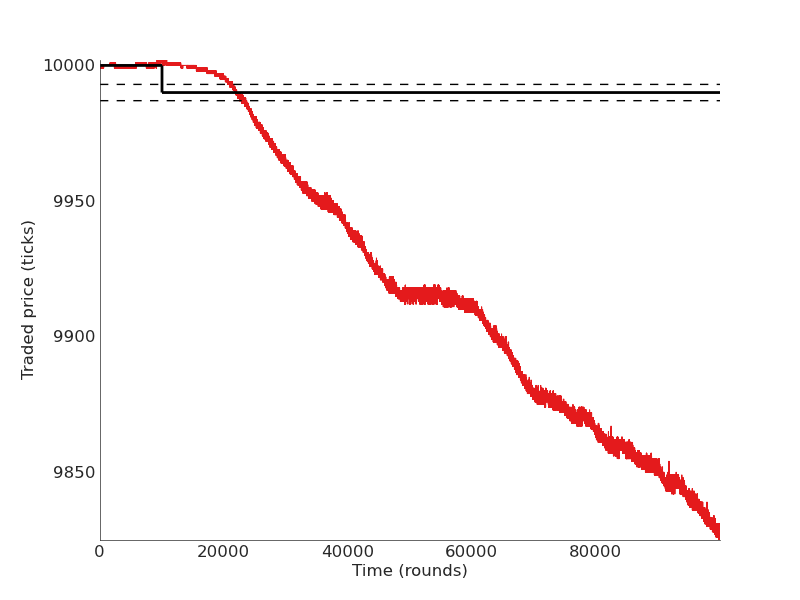
\includegraphics[width=0.5\textwidth]{manually_selected/crashes/shouganai.png}}
	\subcaptionbox{}
     [0.49\linewidth]{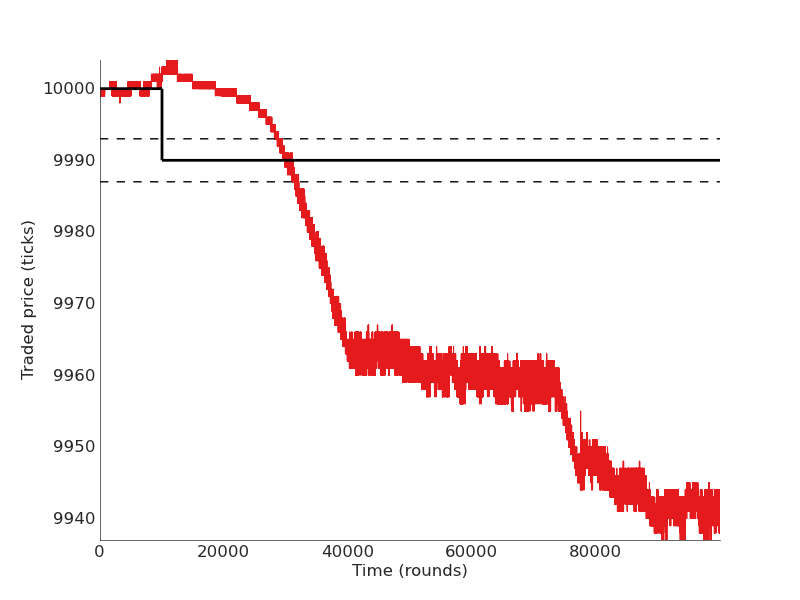
\includegraphics[width=0.5\textwidth]{manually_selected/crashes/slow_but_crash.png}}  
     \caption{Two examples of market crashes}
     \label{}
\end{figure}

\section{Fast market makers causing overvaluation of the stock}
In the previous part it was shown that overvaluation, that is, a discrepancy between the fundamental price and the traded price of the stock, occurs in some markets. 

As was shown in figure XXX, both an increased number of market makers and market makers with lower latencies tended to push the market towards responding slowly to the change in the fundamental price. A slower response means that a discrepancy between the traded price and the true fundamental price persists for longer. In the case of a negative shock ($\fundamentalshocksize < 0$), the fundamental price will be lower than the traded price, which is the same as saying that the stock is overvalued.

While this does not pose a problem in the current market model, it is easy to see how such an inefficiency can be exploited. In the current model, the fast traders do not know the fundamental price, and therefore have no concept of the true value of the stock. Instead the fast agents trade only by observing the order book, whereas it is the slow traders who know the fundamental. However, if fast traders were to obtain information about the fundamental. such a trader would be able to use this knowledge to deliberately trade at below optimal prices, in expectation that the traded price will eventually return to the fundamental price. In the case of a sudden negative shock in the fundamental, such fast fundamentalists would be able to be reasonably safe by short-selling, as aggregated action of all the active fundamentalists will most likely drive the traded price down towards the new and lower fundamental. In the case of a sudden positive shock to the fundamental, the fast fundamentalists would be able to profit by buying up large volumes of stock which they would then sell after the traded price has descended fully or partly to the higher fundamental price. The profit generated by such a strategy would be at the expense of the slow fundamentalist, and is exactly how the fast and informed (e.i., informed of the fundamental price) agents in \cite{} managed to turn a profit. This work has shown that the presence of fast market makers make the scenario assumed in that work more likely to happen.

We find it reasonable to speculate that the increased response time, or prolonged overvaluation of the stock price, is not only due to the nature of the market making strategy, but due to the the market making strategy being used by traders \textit{who are very fast}. When the market makers are very fast, their behavior will be more alike, since they act on almost the same information, and hence their aggregate behavior will combine into a consistent force that has a strong influence on the market. In the field of multi-agent simulation, this phenomenon is known as strategy crowding \cite{macal2005tutorial}, and basically means that agents using similar strategies and/or observe the same environment tend to act in similar ways. In this model. agents generally \textit{do not} observe the same information at the same time, and strategy crowding therefore seems less likely to happen. However, when the agents become fast, the will increasingly start to observe the same information, or at least information which is only very slightly delayed and therefore very similar. This is similar to the argument raised in \cite{}, but whereas the model in that work assumed identical strategies, this work has shown that 

\subsection{Frequency of crashes}
Crashes did not occur often particularly. Even during experiment \deleven, in which the genetic algorithm ended up prioritizing the market response times, and generate a large number of genes with many chartists and very fast market makers, the market had an overshoot of over 25 tick in just less than 0.2\% of the cases\footnote{The simulation was run around $4\cdot 10^5$ times, and 7989 of these had $\overshoot > 25$}. In experiment \dten, not a single case of markets with an overshoot of over 17 ticks was generated. 





